\subsection{Terminálok}

\begin{center}
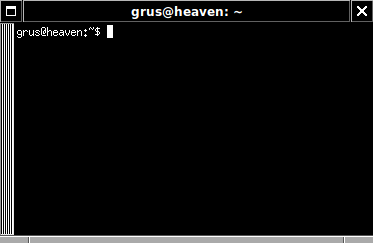
\includegraphics[width=0.6\textwidth]{pics/xterm}

xterm\bigskip


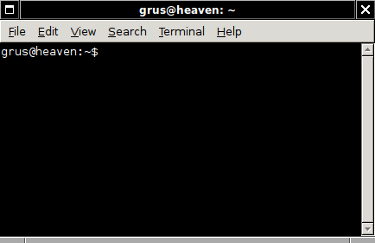
\includegraphics[width=0.6\textwidth]{pics/gnome-terminal}

gnome-terminal\bigskip

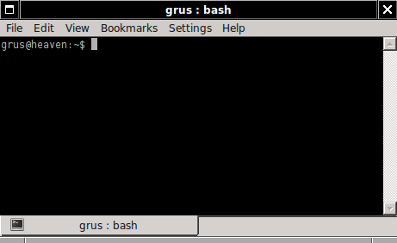
\includegraphics[width=0.6\textwidth]{pics/konsole}

konsole
\end{center}
\pagebreak

\subsection{Alapparancsok}
\subsubsection*{Segítség -- \texttt{man,info}}
\Ovalbox{\large \verb.man. - formázza és kiírja az on-line kézikönyvlapokat }
\medskip

Példa: \texttt{man man} (kilépés: \texttt{q}), man ls (lásd alább)

\begin{lstlisting}
NAME
       ls - list directory contents
SYNOPSIS
       ls [OPTION]... [FILE]...
DESCRIPTION
\end{lstlisting}

%       List information about the FILEs (the current directory by default).  Sort entries alphabetically if none of -cftuvSUX nor --sort is specified.

\subsubsection*{Aktuális könyvtár -- \texttt{pwd, cd}}

\begin{itemize}
\item[]\Ovalbox{\large \verb.pwd. - kiírja az aktuális (munka-) könyvtárat}
	\hfill\texttt{pwd}
	
\item[]\Ovalbox{\large \verb.cd. - az aktuális könyvtár megváltoztatása}
	\hfill\texttt{cd könyvtár}
\end{itemize}

\begin{lstlisting}
joe@localhost:~$ pwd
/home/joe
joe@localhost:~$ cd Documents/
joe@localhost:~/Documents$ pwd
/home/joe/Documents
\end{lstlisting}




\subsubsection*{Létrehozás -- \texttt{mkdir, touch}}
\begin{itemize}
\item[] \Ovalbox{\large \verb.mkdir. - könyvtár létrehozása }
	\hfill \texttt{ mkdir [  kapcsolók  ]   könyvtár}

A \verb.mkdir. Létrehozza a megadott nevű könyvtár(ak)at. 

\medskip

	\textit{Kapcsolók}
	\begin{description}
	\item[-p] Létrehozza a szülőkönyvtárakat is
	 \item[-m jog] A megadott hozzáférési joggal hozza létre a könyvtárakat (később majd ezekről lesz szó)
	\end{description}

\item[] \Ovalbox{\large \verb.touch. - fájl időbélyegének megváltoztatása }
	\hfill\texttt{touch  [-acm][-r   reffájl  |-t   idő  ]   fájl}
	
A \verb.touch. megváltoztatja a megadott fájl(ok) utolsó elérésének és/vagy utolsó módosításának idejét. Ha a fájl nem létezik, a \verb.touch. létrehozza.
\medskip

	\textit{Kapcsolók}
	\begin{description}
	\item[-c, --no-create] Nem hozza létre a fájlokat, ha nem léteznek
	\item[-d, --date= idő] Az idő argumentumot használja az aktuális idő helyett. Ebben lehetnek hónapnevek, időzóna, \texttt{am} vagy \texttt{pm}, stb. 
	\end{description}

\end{itemize}

\begin{lstlisting}
joe@localhost:~/Documents$ ls -lh
total 4.0K
-rw-r--r-- 1 joe joe 827  2011-01-24 01:06 Vicc.txt
joe@localhost:~/Documents$ touch Vicc.txt 
joe@localhost:~/Documents$ ls -lh
total 4.0K
-rw-r--r-- 1 joe joe 827  2011-pics-05 11:44 Vicc.txt
joe@localhost:~/Documents$ mkdir -p newdir/01/pics
joe@localhost:~/Documents$ ls newdir
01
joe@localhost:~/Documents$ ls newdir/01/
pics
\end{lstlisting}




\subsubsection*{Másolás, áthelyezés -- \texttt{cp, mv}}
\begin{itemize}
\item[] \Ovalbox{\large \verb.cp. - fileok másolása} 
	\hfill \texttt{cp [kapcsolók] forrás cél}
\medskip

	\textit{Kapcsolók}
	\begin{description}
	\item[-f] (force) A létező célfájlok törlése
	\item[-i] (interactive) A felhasználó megkérdezése arról, hogy felülírhatók-e a létező célfájlok
	\item[-r,-R] (recursive) A könyvtárak rekurzív másolása, A nem-könytár fájlokat reguláris fájlként másolja 
	\item[-u] (update) Nem másolja azokat a nem-könyvtár fájlokat, amelyeknek azonos vagy újabb módosítási idővel rendelkező célfájlja létezik
	\end{description}


\item[] \Ovalbox{\large \verb.mv. - fileok mozgatása/áthelyezése}
	\hfill\texttt{mv [kapcsolók] forrás cél}
	\medskip
	
	\textit{Kapcsolók}
	\begin{description}
	\item[-f] A létező célfájlok törlése kérdezés nélkül
	\item[-i] A felhasználó megkérdezése arról, hogy felülírhatók-e a létező célfájlok
	\item[-u] Nem mozgatja azokat a nem-könyvtár fájlokat, amelyeknek azonos vagy újabb módosítási idővel rendelkező célfájlja létezik
	\end{description}
\end{itemize}



\subsubsection*{Törlés -- \texttt{rm,rmdir}}
\begin{itemize}
\item[] \Ovalbox{\large rm - állományok eltávolítása}
	\hfill\texttt{rm [ kapcsolók ] fájl(ok)}
	\medskip
	
	\textit{Kapcsolók}
	\begin{description}
	\item[-f] Figyelmen kívül hagyja a nem létező állományokat és nem kérdezi meg a felhasználót
	\item[-i]  Minden fájl eltávolítása előtt megkérdezi a felhasználót, hogy törölheti-e az adott állományt
	\item[-r, -R] A könyvtárak tartalmát rekurzívan törli
	\item[-v] (verbose) Kiírja minden fájl nevét mielőtt törölné
	\end{description}
	
\item[] \Ovalbox{\large rmdir - törli az üres könyvtárakat}
	\hfill\texttt{rmdir [ kapcsolók ] könyvtár(ak)}
	\medskip
	
	\textit{Kapcsolók}
	\begin{description}
	\item[-p] a szülőkönyvtárakat is törli
	%\item[-v] 
	\end{description}
\end{itemize}


\subsubsection*{Kiiratás -- \texttt{cat,less,more}}
\begin{itemize}
\item[] \Ovalbox{\large \verb.cat. - fájlokat fűz össze és kiírja a szabványos kimenetre }
\\
\hspace*{1em}\hfill\texttt{cat [ kapcsolók ] [ file(ok) ]}
	
	
	A cat program minden argumentumként megadott fájlt a szabványos kimenetre ír. Amennyiben nincs fájlnév megadva, vagy a megadott fájlnév a \verb.'-'.-jel, a szabványos bemenetet olvassa. 

\item[] \Ovalbox{\large \verb.more.}
	\hfill\texttt{more [ kapcsolók ] [ -méret ] [ +/ minta ] [ +kezdősor ] [  file(ok) ]}
\item[] \Ovalbox{\large \verb.less.}
	\hfill\texttt{}
	
	A more egy egyszerű szűrőprogram, egy adott szövegből csak egy képernyőnyit mutat. A less egy sok új és hasznos szolgáltatást nyújtó more-emuláció. 
\end{itemize}

	\begin{lstlisting}
	cat fajl.txt
	less fajl.txt
	more fajl.txt
	cat fajl1.txt fajl2.txt
	\end{lstlisting}


\subsubsection*{Filetípus}
\Ovalbox{\large \large\verb.file. - filetípus meghatározása}
	\hfill\texttt{file [ kapcsolók ] [ -f lista ] [ -m bűvösfájl ]  fájl(ok)}\medskip

A file parancs teszteli minden argumentumát és megpróbálja kategorizálni ezeket. %Három teszt sorozatot hajt végre, a következő sorrendben: fájlrendszer tesztek, bűvösszám (magic number) tesztek, és nyelv tesztek. Az első sikeres teszt eredménye határozza meg a program kimenetét.
\bigskip

\begin{lstlisting}
joe@localhost:~/Documents$ ls
Kep001.jpg  Logo.png  newdir  SzegedTreebank.pdf  Vicc.txt
joe@localhost:~/Documents$ file *
Kep001.jpg:         JPEG image data, JFIF standard 1.01, comment: "GIMP"
Logo.png:           PNG image, 180 x 120, 8-bit/color RGBA, non-interlaced
newdir:             directory
SzegedTreebank.pdf: PDF document, version 1.4
Vicc.txt:           UTF-8 Unicode text, with very long lines
\end{lstlisting}


\subsubsection*{Fileok listázása}
\Ovalbox{\large \large \verb.ls. - könytár tartalmának listázása}
	\hfill\texttt{ls [ kapcsoló(k) ] [ file(ok) ]}
	\medskip

	\textit{Kapcsolók}
	\begin{description}
	\item[-1] (egy)  minden sorban csak egy név látszik (egyoszlopos mód)
	\item[-l]  (kis L) hosszú avagy bővített lista
	\item[-a]  a listában a rejtett állományok/könyvtárak is megjelennek 
	
		\emph{Megjegyzés:} rejtett állományok a \verb@.@ (pont)-tal kezdődőek
	\item[-R]  a megadott könyvtár(ak) minden alkönyvtárának és azok teljes tartalmának listázása (rekurzív listázás)
%	\item[-r]  csökkenő sorrend
	\item[-h] olvashatóbb formában írja ki a fileok méreteit 
	\end{description}

%\subsection{Szövegszerkesztők}
%\begin{center}
%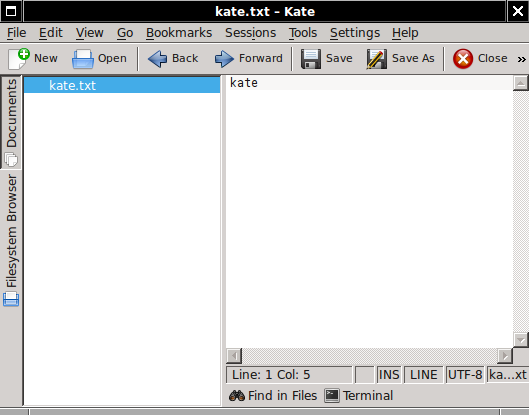
\includegraphics[height=170px]{pics/kate}\hfill
%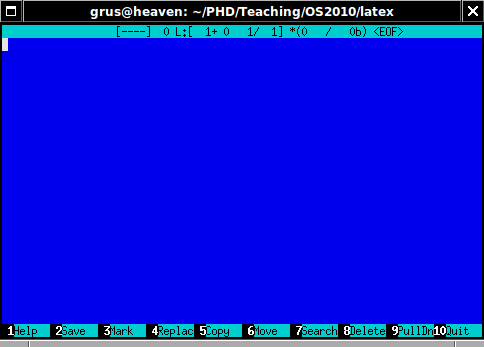
\includegraphics[height=170px]{pics/mcedit}
%\\
%kate\hfill mcedit
%\medskip
%
%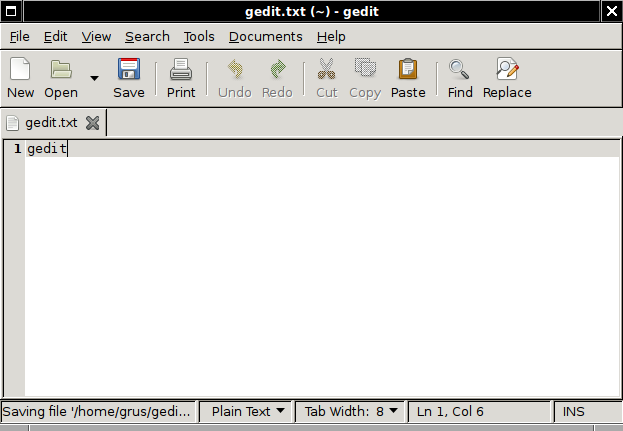
\includegraphics[height=170px]{pics/gedit}\hfill
%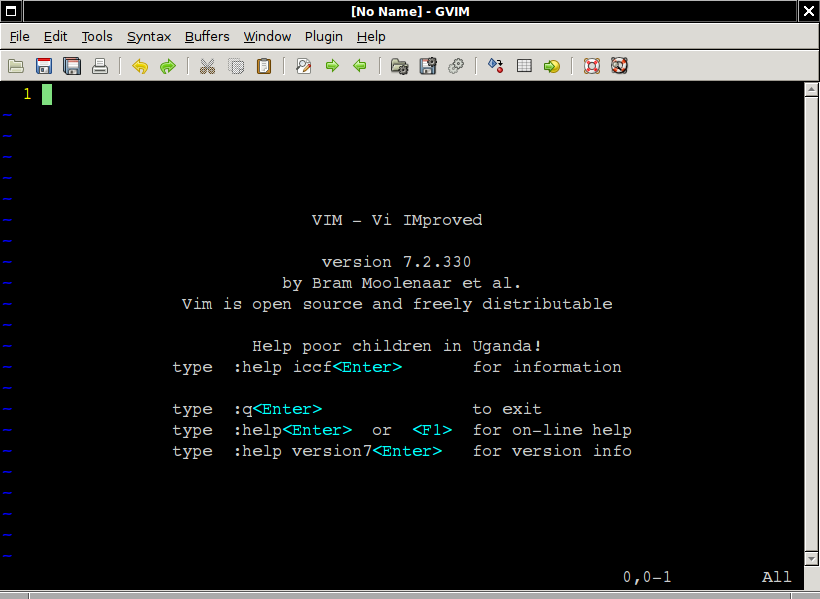
\includegraphics[height=170px]{pics/gvim}
%\\
%gedit \hfill gvim
%\end{center}

\subsection{basename, dirname}
\Ovalbox{\large \large\verb.basename útvonal.}

\begin{quotation}
A könyvtárak neveit eltávolítja a megadott útvonalból (csak az utolsó / utáni állománynév marad meg), majd kiírja az eredményt. Nem ellenőrzi az útvonal valódiságát!
\end{quotation}

\noindent\Ovalbox{\large \large\verb.dirname útvonal.}
\begin{quotation}
Az állomány nevét eltávolítja a megadott útvonalból (csak az utolsó \verb./. előtt álló könyvtárak listája marad meg), majd kiírja az eredményt. Ha az útvonal nem tartalmaz \verb./. jelet, az eredmény a \verb@.@ lesz. Nem ellenőrzi az útvonal valódiságát!
\end{quotation}

%Például:
\begin{lstlisting}
joe@localhost:~$ dirname /usr/bin/nemletezofilenev
/usr/bin
joe@localhost:~$ basename /usr/bin/nemletezofilenev
nemletezofilenev
\end{lstlisting}


%\clearpage

\subsection{Mintaillesztés}
Hasonló felépítésű állomány- vagy könyvtárnevek listájának megadására használhatunk ún. \textit{állománynév mintákat} (filename pattern). Ezek a közönséges karakterek mellett helyettesítő, mintaillesztő avagy Joker-karaktereket is tartalmaznak.
\medskip

\textit{Eredmény:} a mintának megfelelő (mintára illeszkedő) létező nevek szóközökkel tagolt rendezett listája

\subsubsection*{Mintaillesztő karakterek}
\begin{description}
\item{\tt *} tetszőleges karakterekből álló, tetszőlegesen hosszú szó (üres szó is)
\item{\tt ?} egyetlen tetszőleges karakter
\item{\tt[HALMAZ]} A halmaz bármely karakterének egy példánya. A halmazt a karakterek egymás mellé írásával adhatjuk meg.
\item{\tt[ELSŐ-UTOLSÓ]} mint előbb, de itt egy tartományt adunk meg
\item{\tt[\verb.^.HALMAZ]} a halmazban nem szereplő bármely karakter egy példánya
\end{description}

\subsubsection*{Speciális esetek}
Mindig ki kell írni a rejtett állományok/könyvtárak nevének kezdő pont (.) karakterét, ill. könyvtárak esetén a könyvtárnév után a / jelet.

A pont karakter egyéb esetekben nem számít speciálisnak. Néhány program azonban az állománynevekben az utolsó pont utáni részt, az ún. \emph{kiterjesztést} (filename extension) különlegesen kezeli. Ezt általában az állomány tartalma típusának jelzésére használják (pl. kép, video, hang).\bigskip

\noindent\textit{Példák}
\begin{description}
\item{\bf *} az összes nem rejtett állomány és alkönyvtár
\item{\bf */} az összes nem rejtett alkönyvtár
\item{\bf */*} az összes nem rejtett alkönyvtár teljes tartalma
\item{\bf .*} az összes rejtett állomány és alkönyvtár
\item{\bf .*/} az összes rejtett alkönyvtár
\item{\bf *.jpg} a .jpg kiterjesztésű állományok (JPEG formátumú képek)
\item{\bf *.*} az összes nem rejtett állomány és alkönyvtár, amelynek neve tartalmaz legalább egy pontot
\end{description}


%\textit{Példák}
\begin{lstlisting}
joe@localhost:~/dir$ ls -a
.                 ebay_fanshop.png  hello.sh  pepita_sakk.png  ubigraph1.png
..                file.txt          Judy.png  .rejtett1        ubigraph2.png
BatteryLinux.png  final.png         Logo.png  .rejtett
joe@localhost:~/dir$ ls *
BatteryLinux.png  file.txt   hello.sh  Logo.png         ubigraph1.png
ebay_fanshop.png  final.png  Judy.png  pepita_sakk.png  ubigraph2.png
joe@localhost:~/dir$ ls ?ello.sh
hello.sh
joe@localhost:~/dir$ ls ubigraph[12].png
ubigraph1.png  ubigraph2.png
joe@localhost:~/dir$ ls ubigraph[0-9].png
ubigraph1.png  ubigraph2.png
joe@localhost:~/dir$ ls .*
.rejtett1  .rejtett2
joe@localhost:~/dir$ ls *.png
BatteryLinux.png  final.png  Logo.png         ubigraph1.png
ebay_fanshop.png  Judy.png   pepita_sakk.png  ubigraph2.png
\end{lstlisting}


\subsection{Keresés}
\Ovalbox{\large \large\verb.locate. -- mintához illeszkedő fájlokat nyomtat a fájlnév adatbázis(ok)ból}\medskip

\hfill\texttt{locate [ -d   elérési út  ] [ --database=  elérési út  ] [ --version ] [ --help ] minta...}
\medskip

\begin{quotation}
\small
A locate parancs végignézi a megadott fájlnév-adatbázis(oka)t és kinyomtatja azokat a fájl\-ne\-ve\-ket, melyek illeszkednek a mintá(k)ra. A minták tartalmazhatnak shell-stílusú speciális karaktereket is (metakarakterek). Ezek a: '*', '?', és '[]'. A metakarakterek nem kezelik a '/' vagy '.' karaktereket speciálisan, emiatt például a 'foo*bar' minta illeszkedik a 'foo3/bar' karaktersort tartalmazó fájlnévre, hasonlóan a '*duck*' minta is illeszkedik a 'lake/.ducky' karaktersort tartalmazó fájlnevekre. A metakaraktereket tartalmazó mintákat idézőjelek közé kell tenni jelezve, hogy azok nem a parancsértelmezőnek (shell) szólnak. 
\end{quotation}

\noindent\Ovalbox{\large \large\verb.find. -- fájlokat keres egy könyvtárstruktúrában}
	\medskip

	\hfill\texttt{find [útvonal...] [kifejezés] }\medskip


%\begin{quotation}
A find parancs rengeteg kapcsolóval rendelkezik, emellett operátorokat is használhatunk vele, részletesebben lásd \texttt{man find}.
%\end{quotation}
\bigskip

	Álljon itt néhány példa a teljesség igénye  nélkül\footnote{A legtöbb példa a \url{http://linuxbox.hu/find} oldalról származik}.
	Keressünk\dots
	\begin{itemize} 
	\item  \texttt{.jpg} fájlokat az aktuális könyvtárakban így: \verb@find . -name *.jpg@

	\item 20 évnél idősebb állományokat keresünk az aktuális könyvtárban így: \verb@find ./ -mtime +7300@
	\item az utolsó 3 napban módosított állományokat így:	\verb@find . -mtime -3.@

	\item az utolsó 3 napban módosított txt állományokat így: \verb@find . -name '*.txt' -mtime -3@
	
	\item 10000 kbytenál nagyobb állományokat így: \verb@find . -size +10000k@


	\item rc.conf nevű állomány keresése az aktuális könyvtárban
	\begin{lstlisting}
	find . -name "rc.conf" -print
	\end{lstlisting}

	\item ha megtalálta a find az rc.conf nevű állományt akkor azon végre hajtja a chmod utasítást
	\begin{lstlisting}
	find . -name "rc.conf" -exec chmod o+r '{}' \;
	\end{lstlisting}

	\item komplex keresés ami kihagyja az eredményből a *.v vagy .*.v nevű állományokat. Egy kis extra ma\-gya\-rá\-zat: -not negálást jelent, -o a logikai OR műveletet, $\backslash($ a logikai művelet kezdetét jelöli, $\backslash)$ pedig a végét. Egyébként a kihagyott állományok egy verzió kezelő állományai...
	\begin{verbatim}
	find /usr/src -not \( -name "*,v" -o -name ".*,v" \) '{}' \; -print
	\end{verbatim}

	\item keresés a linuxbox szóra a *.html nevű állományokban, állomány név kiiratás találat esetén.
	\begin{lstlisting}
	find . -name "*.html" -exec grep "linuxbox" '{}' \; -print
	\end{lstlisting}

	\item Keresés az aktuális könyvtárból indulva kis és nagybetű nem figyelembe vételével és kihagyni a .svn nevű könyvtárak tartalmát:
	\begin{lstlisting}
	find . -iname "*old*" -a -not -path "*.svn*" -print
	\end{lstlisting}

	Itt igazából az \texttt{-and -or -not} keresési feltételek közti logikai művelet megadás lehetősége a lényeg!

	\end{itemize}

\subsection{Állománynév-kiegészítés}
A hosszabb nevek begépelését könnyíti meg az \emph{állománynév-kiegészítés} (filename completion). A név első pár betűjének beírása után üssük le a \Tab\footnote{Tab} billentyűt. Ha csak egy állomány neve kezdődik így, akkor a név kiegészül. Különben még egyszer üssük le a \Tab-ot, hogy egy listát kapjunk a szóba jöhető nevekről. Ezután folytassuk a gépelést a kívánt karakterrel. Ez a szolgáltatás könyvtár- és programneveknél is működik.



